%%%%%%%%%%%%%%%%%%%% author.tex %%%%%%%%%%%%%%%%%%%%%%%%%%%%%%%%%%%
%
% sample root file for your "contribution" to a contributed volume
%
% Use this file as a template for your own input.
%
%%%%%%%%%%%%%%%% Springer %%%%%%%%%%%%%%%%%%%%%%%%%%%%%%%%%%
% RECOMMENDED %%%%%%%%%%%%%%%%%%%%%%%%%%%%%%%%%%%%%%%%%%%%%%%%%%%
\documentclass[graybox]{svmult}
% choose options for [] as required from the list
% in the Reference Guide
\usepackage{type1cm}        % activate if the above 3 fonts are
                            % not available on your system
%
\usepackage{makeidx}         % allows index generation
\usepackage{graphicx}        % standard LaTeX graphics tool
                             % when including Fig.~files
\usepackage{multicol}        % used for the two-column index
\usepackage[bottom]{footmisc}% places footnotes at page bottom
\usepackage{newtxtext}       % 
\usepackage{newtxmath}       % selects Times Roman as basic font
% see the list of further useful packages
% in the Reference Guide
%\makeindex             % used for the subject index
                       % please use the style svind.ist with
                       % your makeindex program
%%%%%%%%%%%%%%%%%%%%%%%%%%%%%%%%%%%%%%%%%%%%%%%%%%%%%%%%%%%%%%%%%%%%%%%%%%%%%%%%%%%%%%%%%
\usepackage{listings}
\lstset{%
 language={C},
% basicstyle={\scriptsize},%
% identifierstyle={\scriptsize},%
 basicstyle={\small},%
 identifierstyle={\small},%
% commentstyle={\small\itshape},%
%commentstyle={\scriptsize},%
commentstyle={\small},%
 keywordstyle={\small\bfseries},%
 ndkeywordstyle={\small},%
stringstyle={\small\ttfamily},
 frame={tb},
 breaklines=true,
 columns=[l]{fullflexible},%
 numbers=left,%
 xrightmargin=1zw,%
 xleftmargin=1.5zw,%
 numberstyle={\small},%
 stepnumber=1,
 numbersep=1zw,%
% lineskip=-0.1ex%
}
%%%%%%%%%%%%%%%%%%%%%%%%%%%%%%%%%%%%%%%%%%%%%%%%%%%%%%%%%%%%%%%%%%%%%%%%%%%%%%%%%%%%%%%%%
\begin{document}
\title*{Implementation and Performance Evaluation of Omni compiler}
% Use \titlerunning{Short Title} for an abbreviated version of
% your contribution title if the original one is too long
\author{Masahiro Nakao and Hitoshi Murai}
% Use \authorrunning{Short Title} for an abbreviated version of
% your contribution title if the original one is too long
\institute{Masahiro Nakao \at RIKEN Center for Computational Science, 7-1-26 Minatojima-minami-machi, Chuo-ku, Kobe, Hyogo 650-0047, Japan, \email{masahiro.nakao@riken.jp}
\and Hitoshi Murai \at RIKEN Center for Computational Science, 7-1-26 Minatojima-minami-machi, Chuo-ku, Kobe, Hyogo 650-0047, Japan \email{h-murai@riken.jp}}
%
% Use the package "url.sty" to avoid
% problems with special characters
% used in your e-mail or web address
%
\maketitle

\abstract*{This chapter describes implementation and performance evaluation of Omni compiler, which is a compiler for XcalableMP.
For performance evaluation, this chapter also explains how to implement the HPC Challenge benchmark, which is a benchmark suite for an  HPC parallel language.
The results show that the performance of XMP  is comparable to that of MPI in many cases.}

\abstract{This chapter describes implementation and performance evaluation of Omni compiler, which is a compiler for XcalableMP.
For performance evaluation, this chapter also explains how to implement the HPC Challenge benchmarks, which is a benchmark suite for an HPC parallel language.
The results show that the performance of XMP  is comparable to that of MPI in many cases.}

\section{Overview}
Omni compiler is a source-to-source compiler that translates a sequential code in C and Fortran with XcalableMP (XMP), XcalableACC (XACC), and OpenACC directives into a parallel code\cite{omni}.
The translated parallel code is compiled with a native compiler linked with Omni compiler runtime library. 
Omni compiler has been developed by Programming Environment Research Team of RIKEN Center for Computational Science\cite{pro-env} and HPCS laboratory\cite{hpcs} of University of Tsukuba in Japan.

%%%%%%%%%%%%%%%%%%%%%%%%%%%%%%%%%%%%%%%%%%%%%%%%%%%%%%%%%%%%%%%%%%%%%%%%%%%%
\section{Implementation}
\subsection{Operation Flow}
In Omni compiler,
XcodeML\cite{xcodeml} is used to analyze a code in an intermediate code format of XML expression.
Fig.~\ref{fig:xcodeml} shows an operation flow of Omni compiler.
Firstly, Omni compiler translates directives in a user code into the runtime functions. 
If necessary, a code besides the directives is also modified. 
Secondly, a native compiler (e.g., gcc or Intel) compiles the translated code and creates an execution binary with linking to Omni compiler runtime library.
The runtime library uses MPI in XMP, and CUDA in OpenACC, and both MPI and CUDA in XACC.
As for XMP, 
Omni compiler may create better runtime libraries by adding a onesided communication library to MPI, which is described in Chapter 3.
%
\begin{figure}[h]
\sidecaption
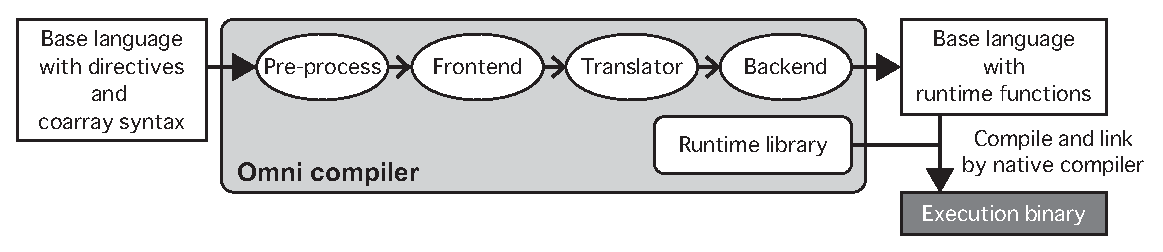
\includegraphics[scale=.6]{img/flow.eps}
\caption{Operation Flow of Omni compiler\cite{omni}} \label{fig:xcodeml}
\end{figure}
%%%%%%%%%%%%%%%%%%%%%%%%%%%%%%%%%%%%%%%%%%%%%%%%%%%%%%%%%%%%%%%%%%%%%%%%%%%%
\subsection{Example of Code Translation}
This section describes how Omni compiler translates a user code for the global-view memory model.
A code translation for the local-view memory model is described in Chapter 3.

\subsubsection{Distributed array}
Fig.~\ref{fig:translation-align} shows an XMP example code using an {\bf align} directive to declare a distributed array {\it a[][]}. 

Firstly, Omni compiler deletes a declaration of a local array {\it a[][]} and the {\bf align}  directive.
Next, Omni compiler creates a descriptor {\it \_XMP\_DESC\_a} by a function {\tt \_XMP\_init\_array\_desc()} to set information of the distributed array. 
Omni compiler also adds a function {\tt \_XMP\_alloc\_array()} to allocate memory for the distributed array, and it sets values in an address {\it \_XMP\_ADDR\_a} and a leading dimension {\it \_XMP\_ACC\_a\_0}.
Note that a multidimensional distributed array is expressed as a one-dimensional array in the translated code
since the size of each dimension of the array may be determined dynamically.

\begin{figure}[h]
\sidecaption
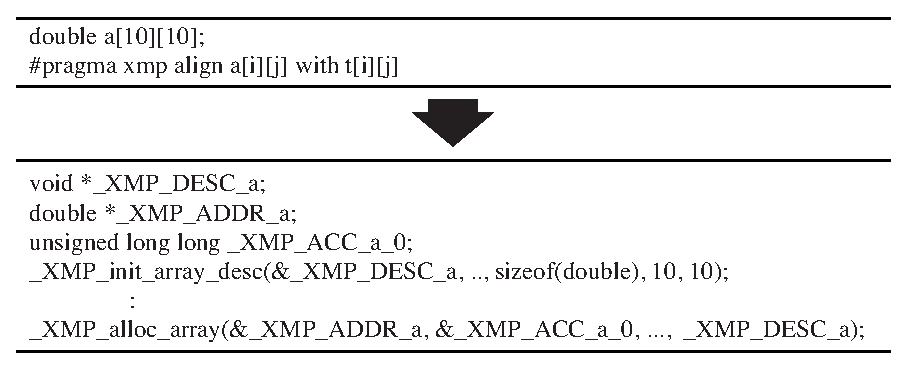
\includegraphics[scale=.75]{img/translation-align.eps}
\caption{Code translation of align directive} \label{fig:translation-align}
\end{figure}
%%%%%%%%%%%%%%%%%%%%%%%%%%%%%%%%%%%%%%%%%%%%%%%%%%%%%%%%%%%%%%%%%%%%%%%%%%%%
\subsubsection{Loop statement}
Fig.~\ref{fig:translation-loop} shows an XMP example code using a {\bf loop} directive to parallelize the following nested loop statement depending on the template {\it t}. 
Each dimension of {\it t} is distributed onto two nodes, which is omitted there.

\begin{figure}[h]
\sidecaption
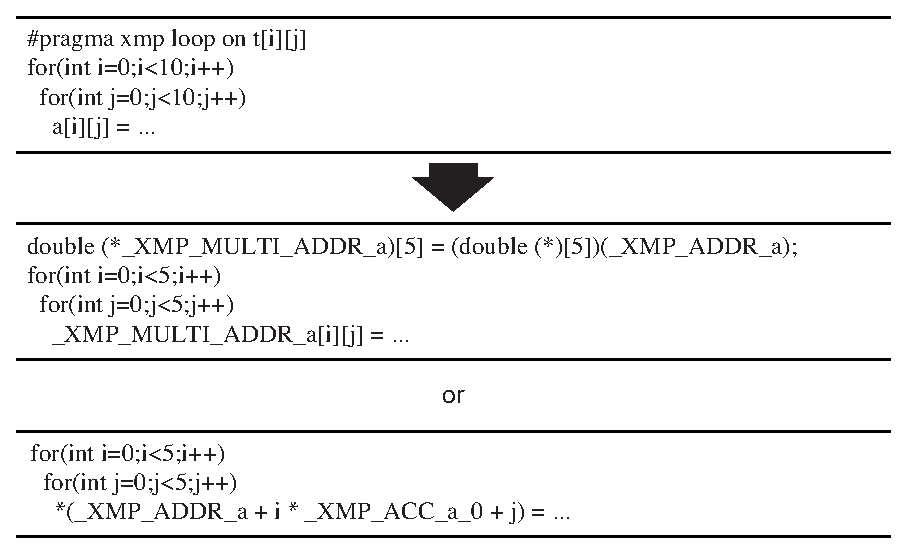
\includegraphics[scale=.75]{img/translation-loop.eps}
\caption{Code translation of loop directive} \label{fig:translation-loop}
\end{figure}

In the translated code above,
a pointer {\it \_XMP\_MULTI\_ADDR\_a} is used which has the size of each dimension as a head pointer of the distributed array {\it a[][]}.
To improve performance, operations in a loop statement are performed using the pointer\cite{ixpug}.
Note that this pointer can be used when the number of elements in each dimension of a distributed array is divisible by the number of nodes,
If the condition is not met, a one-dimensional pointer  {\it \_XMP\_ADDR\_a}  and  {\it \_XMP\_ACC\_a\_0} are used as shown in the translated code below.

Moreover, because values in ending conditions of the loop statement ({\it i} < 10, {\it j} < 10) are constants in a pre-translated code and are divisible by the number of nodes,
the values are translated to constants  ({\it i} < 5, {\it j} < 5) automatically.
If the values are variables in the pre-translated code or not divisible by the number of nodes,
the runtime function is inserted just before the loop statement to calculate values for ending conditions.
The  calculated values are set in newly created variables.
%%%%%%%%%%%%%%%%%%%%%%%%%%%%%%%%%%%%%%%%%%%%%%%%%%%%%%%%%%%%%%%%%%%%%%%%%%%%
\subsubsection{Communication}
Fig.~\ref{fig:translation-bcast} shows an XMP example code using a {\bf bcast} directive to broadcast a local array {\it b}. 
Basically translations of communication directives are simple.
The runtime functions call MPI functions directly.
\begin{figure}[h]
\sidecaption
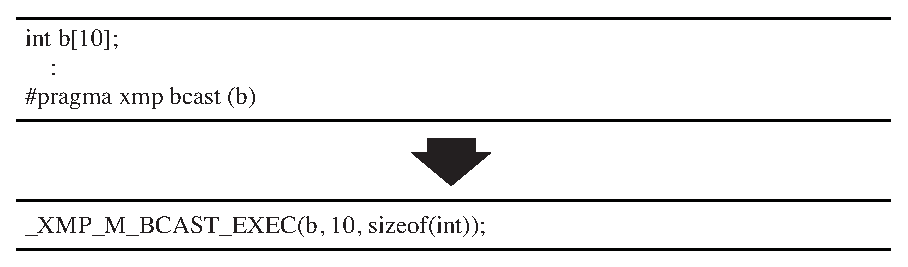
\includegraphics[scale=.75]{img/translation-bcast.eps}
\caption{Code translation of bcast directive} \label{fig:translation-bcast}
\end{figure}
%%%%%%%%%%%%%%%%%%%%%%%%%%%%%%%%%%%%%%%%%%%%%%%%%%%%%%%%%%%%%%%%%%%%%%%%%%%%
\section{Installation}
This section describes how to install the latest Omni compiler version 1.3.2.
Omni compiler is installed by a general installation method on UNIX ( {\tt ./configure; make; make install} ).
When executing {\tt ./configure} without options, only XMP is installed. 
When installing OpenACC and/or XACC, 
it is required for some options to ``{\tt ./configure}'', which is described in Section \ref{sec:optional}.
%%%%%%%%%%%%%%%%%%%%%%%%%%%%%%%%%%%%%%%%%%%%%%%%%%%%%%%%%%%%%%%%%%%%%%%%%%%%
\subsection{Overview}
We provide two versions of Omni compiler, the one is ``stable version'' and the other is ``nightly build version''.
While the stable version is a so-called official version that has a version number, 
the nightly build version is a trial version that is released at midnight on our website (\url{\textcolor{blue}{https://omni-compiler.org}}).
Omni compiler is developed in GitHub repository\cite{github}.
Our web server gets the source code from the GitHub repository and generates the nightly build version every day.
%%%%%%%%%%%%%%%%%%%%%%%%%%%%%%%%%%%%%%%%%%%%%%%%%%%%%%%%%%%%%%%%%%%%%%%%%%%%
\subsection{Get source code}
\subsubsection{From GitHub}
Please visit the GitHub repository (\url{\textcolor{blue}{https://github.com/omni-compiler/omni-compiler}}) which provides only nightly build version.
Otherwise, please execute the following {\tt git} command.

\begin{svgraybox}
\$ git clone {-}{-}recursive https://github.com/omni-compiler/omni-compiler.git
\end{svgraybox}
Note that the source code of Omni compiler does not contain that of XcodeML, so the  {\tt {-}{-}recursive} option is required.
As a supplement, 
XcodeML is also developed in the GitHub repository (\url{\textcolor{blue}{https://github.com/omni-compiler/xcodeml-tools}}).

\subsubsection{From our website}
Please visit our website (\url{\textcolor{blue}{https://omni-compiler.org}}) which provides packages of stable version and nightly build version.
The package of nightly build version is generated every midnight around 12:00 AM (JST) if the latest GitHub repository was updated yesterday.
These packages contain XcodeML.

\subsection{Software dependency}
Before installation of Omni compiler, the following software must be installed.
\begin{svgraybox}
yacc, lex, C Compiler (C99 or over), Fortran Compiler (Fortran 2008 or over), Java Compiler, MPI (version 2 or over), libxml2, make
\end{svgraybox}

%%%%%%%%%%%%%%%%%%%%%%%%%%%%%%%%%%%%%%%%%%%%%%%%%%%%%%%%%%%%%%%%%%%%%%%%%%%%
\subsection{General installation}
This section explains how to install Omni compiler in a general Unix environment.

\subsubsection{Build and install}

\begin{svgraybox}
\$ ./configure {-}{-}prefix=(INSTALL PATH)\\
\$ make\\
\$ make install
\end{svgraybox}
%
%\begin{warning}{Attention}
%(INSTALL PATH) can not be set to a directory of the source code of Omni compiler.
%\end{warning}

\subsubsection{Set PATH}
\begin{itemize}
\item bash and zsh
\begin{svgraybox}
\$ export PATH=(INSTALL PATH)/bin:\$PATH
\end{svgraybox}
\item csh and tcsh
\begin{svgraybox}
\% setenv PATH (INSTALL PATH)/bin:\$PATH
\end{svgraybox}
\end{itemize}

\subsection{Optional installation}\label{sec:optional}
\subsubsection{OpenACC}
Please add ``{\tt {-}{-}enable-openacc}'' and ``{\tt {-}{-}with-cuda=(CUDA PATH)}'' options to ``{\tt ./configure}''.

\begin{svgraybox}
\$ ./configure {-}{-}enable-openacc {-}{-}with-cuda=(CUDA PATH)\\
\$ make\\
\$ make install
\end{svgraybox}

It may be possible to generate a more suitable runtime library by adding options to ``{\tt nvcc}'' command, 
which is used to generate the runtime library for OpenACC and XACC. 
In that case, please also add the ``{\tt {-}{-}with-gpu-cflags=(NVCC CFLAGS)}'' option.

\begin{svgraybox}
\$ ./configure {-}{-}enable-openacc {-}{-}with-cuda=(CUDA PATH) {-}{-}with-gpu-cflags=(NVCC CFLAGS)\\
\$ make\\
\$ make install
\end{svgraybox}

\subsubsection{XcalableACC}
Please add ``{\tt {-}{-}enable-openacc {-}{-}enable-xacc}'' to ``{\tt ./configure}''.

\begin{svgraybox}
\$ ./configure {-}{-}enable-openacc {-}{-}enable-xacc\\
\$ make\\
\$ make install
\end{svgraybox}
As with OpenACC, if necessary,
please add the ``{\tt {-}{-}with-cuda=(CUDA PATH)}'' and ``{\tt {-}{-}with-gpu-cflags=(NVCC CFLAGS)}'' options to ``{\tt ./configure}''.

\subsubsection{Onesided library}
Omni compiler may generate a better runtime library by a onesided library for XMP. 
Omni compiler supports the following onesided libraries.

\begin{itemize}
\item Fujitsu MPI Extended RDMA (FJRDMA)\\
It is low-level communication layer for Fujitsu machines (e.g. the K computer, FX100, and FX10).
When using it, please specify a target machine to ./configure. (e.g. ``{\tt \$ ./configure {-}{-}target=FX100-linux-gnu}'')
\item GASNet\cite{gasnet}\\
It is a onesided communication library developed by U.C. Berkeley. 
When using it, please specify ``install path of GASNet'' and ``its conduit'' to ./configure. (e.g. {\tt \$ ./configure {-}{-}with-gasnet=/usr {-}{-}with-gasnet-conduit=ibv})
\item MPI version 3\\
Omni compiler automatically selects MPI version 3 under the following conditions.
\begin{itemize}
\item MPI implementation supports MPI version 3
\item Specifying neither FJRDMA nor GASNet.
\end{itemize}
\end{itemize}
%%%%%%%%%%%%%%%%%%%%%%%%%%%%%%%%%%%%%%%%%%%%%%%%%%%%%%%%%%%%%%%%%%%%%%%%%%%%
\section{Creation of execution binary}
This section describes how to create an execution binary from a code with XMP, XACC, and OpenACC directives, and how to execute it.
Note that Omni compiler supports only C language for OpenACC.
%%%%%%%%%%%%%%%%%%%%%%%%%%%%%%%%%%%%%%%%%%%%%%%%%%%%%%%%%%%%%%%%%%%%%%%%%%%%
\subsection{Compile}
\begin{itemize}
\item XMP in C language
\begin{svgraybox}
\$ xmpcc a.c
\end{svgraybox}
\item XMP in Fortran
\begin{svgraybox}
\$ xmpf90 a.f90
\end{svgraybox}
\item XACC in C language
\begin{svgraybox}
\$ xmpcc -xacc a.c
\end{svgraybox}
\item XACC in Fortran
\begin{svgraybox}
\$ xmpf90 -xacc a.f90
\end{svgraybox}
\item OpenACC in C language
\begin{svgraybox}
\$ ompcc -acc a.c
\end{svgraybox}
\end{itemize}

A native compiler finally compiles the code translated by Omni compiler.
Thus, all compile options of XMP are passed to the native compiler. 
For example, when using the optimization option ``{\tt -O2}'', it is passed to the native compiler.

\begin{svgraybox}
\$ xmpcc -O2 a.c
\end{svgraybox}

%%%%%%%%%%%%%%%%%%%%%%%%%%%%%%%%%%%%%%%%%%%%%%%%%%%%%%%%%%%%%%%%%%%%%%%%%%%%
\subsection{Execution}
\subsubsection{XcalableMP and XcalableACC}
Because the runtime libraries of XMP and XACC use MPI, 
 a program is executed via an MPI execution command (e.g. ``{\tt mpiexec}'').
However, when using GASNet, 
 a program is executed via a GASNet execution command (e.g. ``{\tt gasnetrun\_ibv}'').

\begin{svgraybox}
\$ mpiexec -n 2 ./a.out
\end{svgraybox}
\begin{svgraybox}
\$ gasnetrun\_ibv -n 2 ./a.out
\end{svgraybox}

\subsubsection{OpenACC}
\begin{svgraybox}
\$ ./a.out
\end{svgraybox}
%%%%%%%%%%%%%%%%%%%%%%%%%%%%%%%%%%%%%%%%%%%%%%%%%%%%%%%%%%%%%%%%%%%%%%%%%%%%
\subsection{Cooperation with profiler}
In order to improve the  performance of an application, it is useful to take a profile.
Omni compiler has a function to cooperate with Scalasca\cite{scalasca} and tlog which are profiling tools. 
The function can profile the  execution of XMP directives. 
Note that the function supports only the XMP in C language now.

\subsubsection{Scalasca}\label{sec:scalasca}
Scalasca is an opensource software  that measures and analyzes the runtime behaviors. 

When profiling all XMP directives that exist in code, please add the ``{\tt {-}{-}profile scalasca}'' option to a compile command.

\begin{svgraybox}
\$ xmpcc {-}{-}profile scalasca a.c
\end{svgraybox}

When profiling selected XMP directives there, 
please add the ``{\tt profile}'' clause to the directives and the ``{\tt {-}{-}selective-profile scalasca}'' option to a compile command.

\begin{svgraybox}
\#pragma xmp bcast (a) profile
\end{svgraybox}

\begin{svgraybox}
\$ xmpcc {-}{-}selective-profile scalasca a.c
\end{svgraybox}

Fig.~\ref{fig:scalasca} shows an example of profiling by Scalasca.

\begin{figure}[h]
\sidecaption
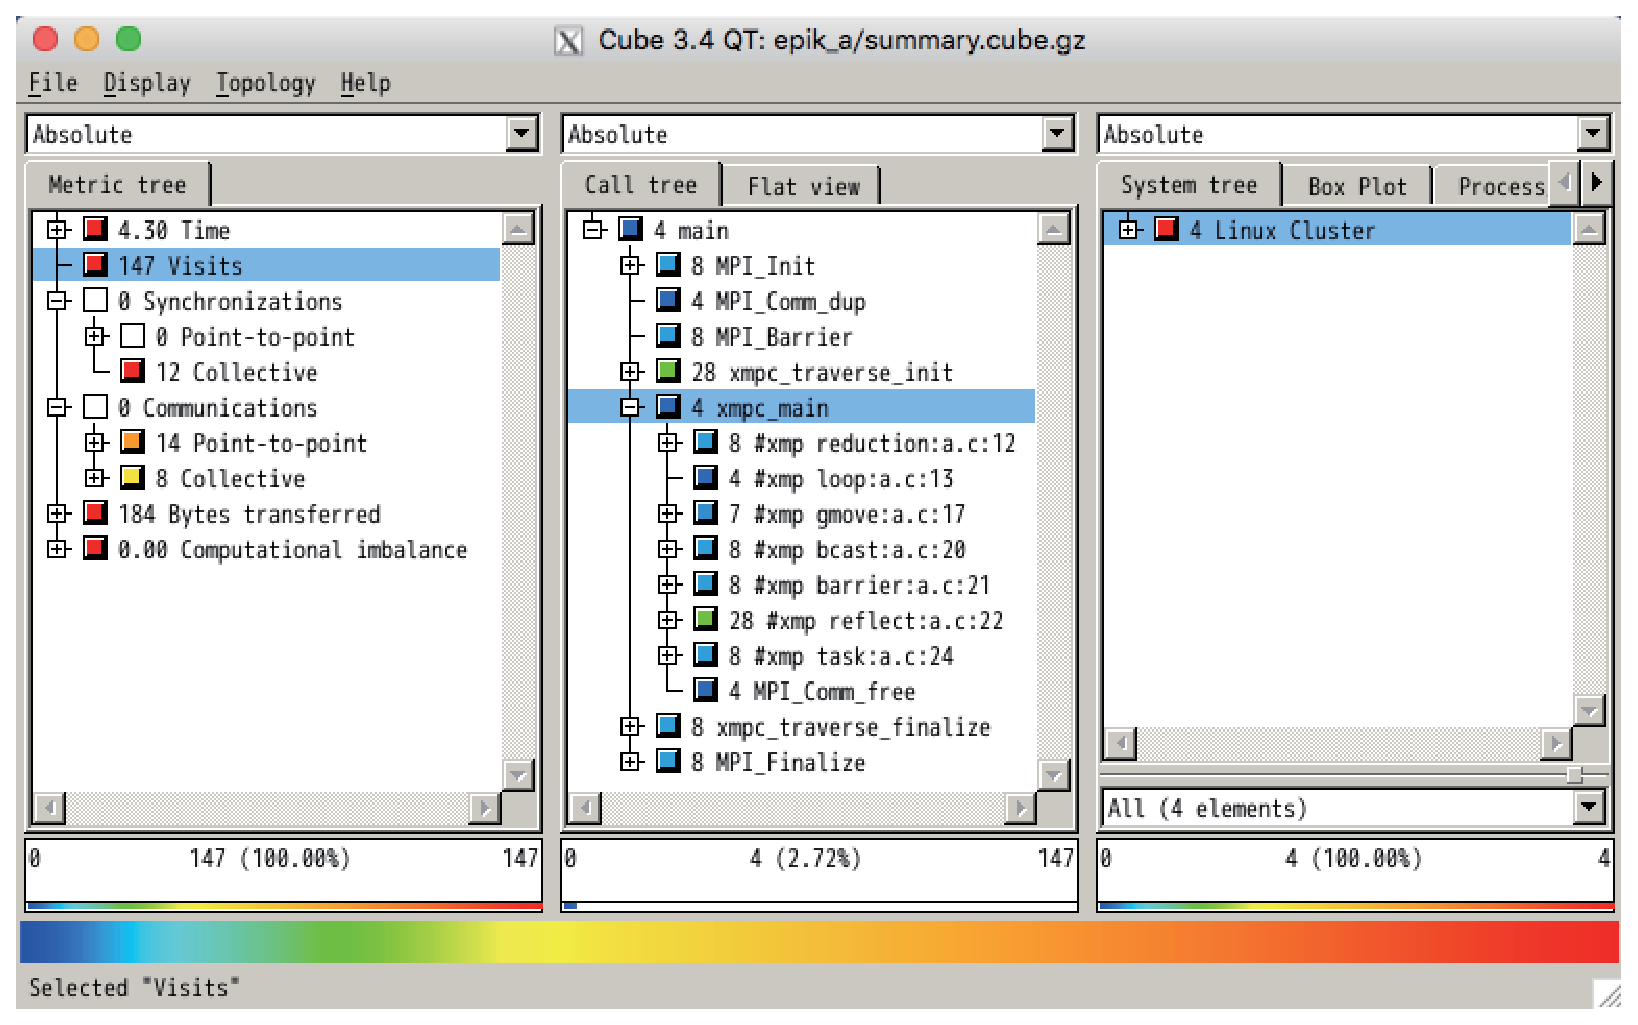
\includegraphics[scale=.43]{img/scalasca.eps}
\caption{Profile by Scalasca\cite{omni}} \label{fig:scalasca}
\end{figure}

\subsubsection{tlog}
Omni compiler package contains tlog that measures executing time of the XMP directives.

When profiling all XMP directives that exist in code, please add the ``{\tt {-}{-}profile tlog}'' option to a compile command.

\begin{svgraybox}
\$ xmpcc {-}{-}profile tlog a.c
\end{svgraybox}

When profiling selected XMP directives there, 
please add the ``{\tt profile}'' clause to the directives as in Section \ref{sec:scalasca} and  the ``{\tt {-}{-}selective-profile tlog}'' option to a compile command.

\begin{svgraybox}
\$ xmpcc {-}{-}selective-profile tlog a.c
\end{svgraybox}

After executing a program,
tlog generates a file ``{\tt trace.log}'' which stores profiling results. 
To open the result, 
please use the ``{\tt tlogview}'' command.
Fig.~\ref{fig:scalasca} shows an example of profiling by tlog.

\begin{svgraybox}
\$ tlogview trace.log
\end{svgraybox}

\begin{figure}[h]
\sidecaption
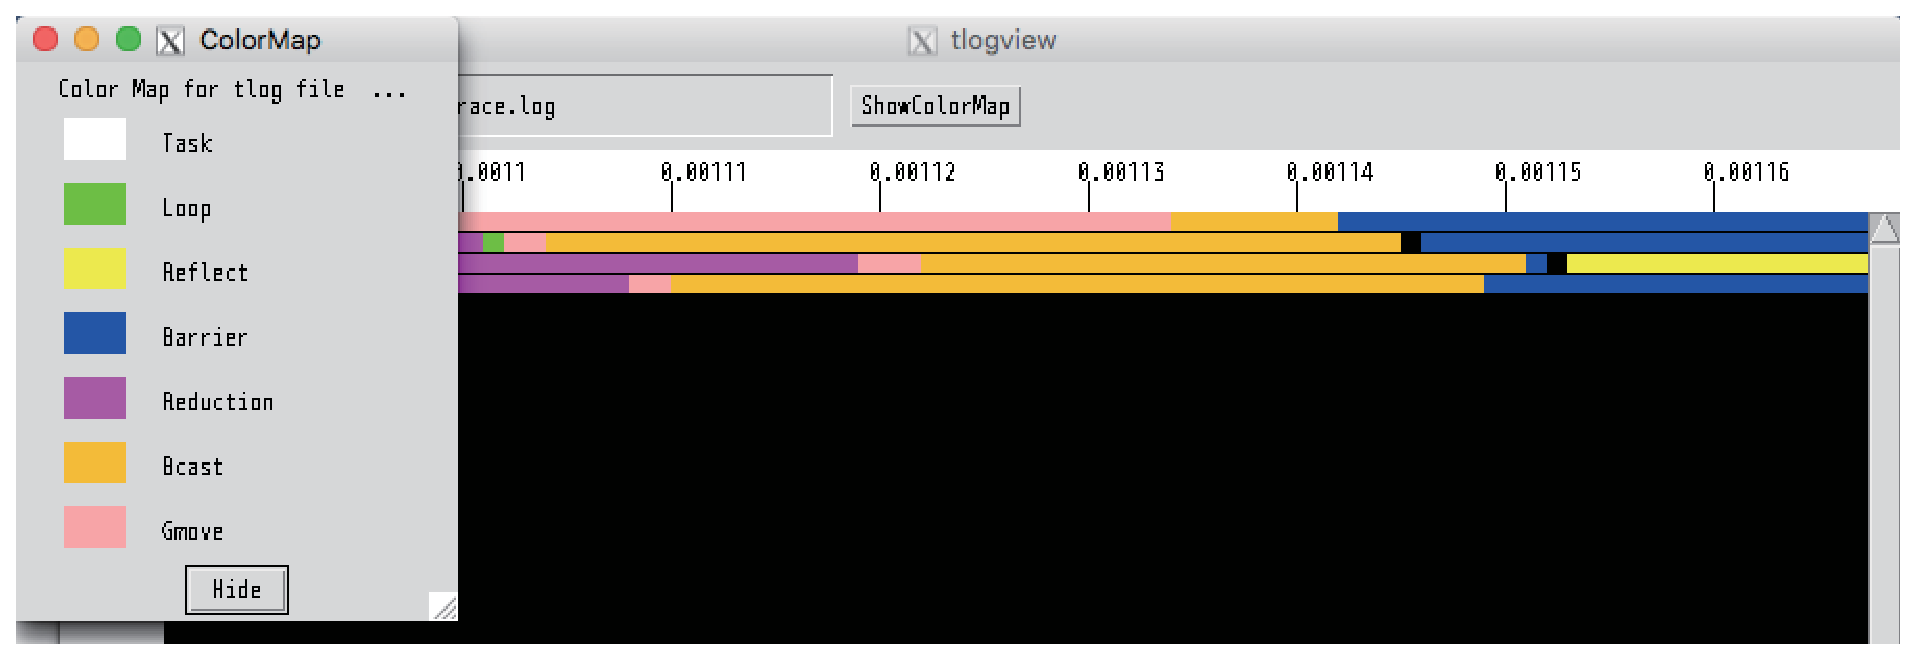
\includegraphics[scale=.365]{img/tlog.eps}
\caption{Profile by tlog\cite{omni}} \label{fig:tlog}
\end{figure}
%%%%%%%%%%%%%%%%%%%%%%%%%%%%%%%%%%%%%%%%%%%%%%%%%%%%%%%%%%%%%%%%%%%%%%%%%%%%
\section{Performance Evaluation}
In order to evaluate the performance of XMP,
we implement the HPC Challenge (HPCC) benchmark\cite{hpcc}, namely, 
EP STREAM Triad (STREAM), High Performance Linpack (HPL), Global fast fourier transform (FFT), and RandomAccess\cite{hpca}.
While the HPCC benchmark is used to evaluate multiple attributes of HPC systems, 
the benchmark is also useful to evaluate the properties of a parallel language.
The HPCC benchmark was used at the HPCC Award Competition\cite{hpcc-a}. 
The HPCC Award Competition consists of two classes. 
While the purpose of class 1 is to evaluate the performance of a machine, 
the purpose of class 2 is to evaluate both the productivity and performance of a parallel programming language.
XMP won the class 2 prizes in 2013 and 2014.

%%%%%%%%%%%%%%%%%%%%%%%%%%%%%%%%%%%%%%%%%%%%%%%%%%%%%%%%%%%%%%%%%%%%%%%%%%%%
\subsection{Experimental environment}
For performance evaluation, 
this section uses 16,384 compute nodes on the K computer and 128 compute nodes on a Cray CS300 system named ``the COMA system''.
Table~\ref{tab:spec-k} and \ref{tab:spec-coma} show the hardware specifications and software environments. 

\begin{table}[h]
\caption{Experimental environment for the K computer}\label{tab:spec-k}
\begin{tabular}{l|l}
\hline\noalign{\smallskip}
~CPU~        & ~SPARC64 VIIIfx 2.0GHz, 8Cores \\
~Memory~  & ~DDR3 SDRAM 16GB, 64GB/s \\
~Network~  & ~Torus fusion six-dimensional mesh/torus network, 5GB/s $\times$ 10 \\
~Library~    & ~Fujitsu Compiler K-1.2.0-19, Fujitsu MPI K-1.2.0-19, Fujitsu SSLII K-1.2.0-19\\
\noalign{\smallskip}\hline\noalign{\smallskip}
\end{tabular}
\end{table}

\begin{table}[h]
\caption{Experimental environment for the COMA system}\label{tab:spec-coma}
\begin{tabular}{l|l}
\hline\noalign{\smallskip}
~CPU~        & ~Xeon E5-2670v2, 2.5GHz  (Turbo Boost 3.3GHz), 10Cores $\times$ 2CPUs \\
~Memory~  & ~DDR3 SDRAM 64GB, 119.4GB/s (= 59.7GB/s $\times$ 2CPUs) \\
~Network~  & ~InfiniBand FDR, fat-tree, 7GB/s \\
~Library~    & ~Intel Compiler 15.0.5, Intel MPI 5.1.1, GASNet 1.26.0, Intel MKL 11.2.4\\
\noalign{\smallskip}\hline\noalign{\smallskip}
\end{tabular}
\end{table}

For comparison purposes, this section also evaluates the  HPCC benchmark in C language and MPI library. 
We execute STREAM, HPL, and FFT with eight threads per process on each CPU of the K computer, 
and with ten threads per process on each CPU of the COMA system. 
Since RandomAccess is not parallelized with threads and can be executed by the power of only two processes, 
we execute it with eight processes on each CPU of both systems.

The specification of HPCC Award Competition class 2 defines the minimum problem size for each benchmark. 
While the main array of HPL should occupy at least half of the system memory, 
the main arrays of STREAM, FFT, and RandomAccess should occupy at least a quarter of the system memory. 
We set each problem size to be equal to the minimum size.
As for coarray syntax, Omni compiler uses FJRDMA on the K computer and uses GASNet on the COMA system.
%%%%%%%%%%%%%%%%%%%%%%%%%%%%%%%%%%%%%%%%%%%%%%%%%%%%%%%%%%%%%%%%%%%%%%%%%%%%
\subsection{EP STREAM Triad}
\subsubsection{Design}
STREAM measures the memory bandwidth to use simple vector kernel ({$a \leftarrow b + \alpha c$}).
STREAM is so straightforward that its kernel does not require communication.
%Our implementation only aggregates a performance result that each node obtains.
%%%%%%%%%%%%%%%%%%%%%%%%%%%%%%%%%%%%%%%%%%%%%%%%%%%%%%%%%%%%%%%%%%%%%%%%%%%%
\subsubsection{Implementation}
\begin{figure}[h]
\begin{lstlisting}
#pragma xmp nodes p[*]
double a[N], b[N], c[N], scalar;
...
for(k=0;k<TIMES;k++){
#pragma xmp barrier
  times[k] = -xmp_wtime();

#pragma loop xfill
#pragma loop noalias
#pragma omp parallel for
  for (i=0; i<N; i++)
    a[i] = b[i] + scalar * c[i];

#pragma xmp barrier
  times[k] += xmp_wtime();
}
double performance = local_performance(time, TIMES, N);
#pragma xmp reduction(+:performance)
\end{lstlisting}
\caption{Part of the STREAM code\cite{hpca}}\label{fig:code-stream}
\end{figure}

Fig.~\ref{fig:code-stream} shows a part of the STREAM code.
In line 1,
the {\bf node} directive declares a node array {\it p} to parallelize the program.
In line 2, normal arrays {\it a[]}, {\it b[]}, and {\it c[]}, and a scalar value {\it scalar} are declared.
In lines 5 and 14, the {\bf barrier} directive is inserted before {\tt xmp\_wtime()} to measure time.
The directives of lines 8--9 are optimization directives for the Fujitsu compiler.
While the {\bf \#pragma loop xfill} ensures one cache line to store write-only data,
the {\bf \#pragma loop noalias} indicates that different pointer variables can not possibly indicate the same storage area.
These optimization directives are used on only the K computer.
In lines 10--12, STREAM kernel is parallelized by the OpenMP {\bf parallel} directive.
% and are also useful for the MPI implementation.
In line 17, {\bf local\_performance()} calculates the performance on each node locally.
In line 18, the {\bf reduction} directive performs a reduction operation among nodes to calculate the total performance.
%%%%%%%%%%%%%%%%%%%%%%%%%%%%%%%%%%%%%%%%%%%%%%%%%%%%%%%%%%%%%%%%%%%%%%%%%%%%
\subsubsection{Evaluation}
\begin{figure}[h]
\sidecaption
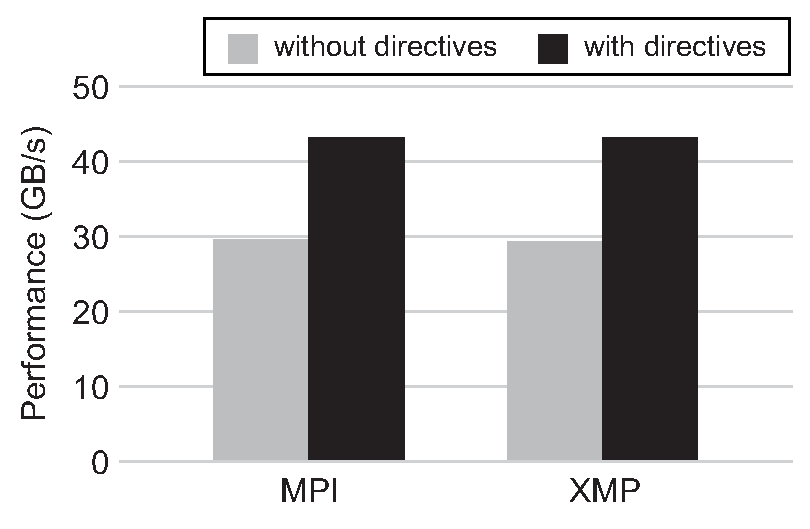
\includegraphics[scale=0.5,clip]{img/result-stream-pre.eps}
\caption{Preliminary evaluation of STREAM\cite{hpca}}\label{fig:result-stream-pre}
\end{figure}

First of all,
in order to consider the effectiveness of {\bf \#pragma loop xfill} and {\bf \#pragma loop noalias},
we evaluate STREAM with and without these directives on a single node of the K computer.
We also insert these directives into the MPI implementation for evaluation.
Fig.~\ref{fig:result-stream-pre} shows that the performance results with these directives are about 1.46 times better than those without the directives.
Therefore, we use the directives in next evaluations.

\begin{figure}[h]
\sidecaption
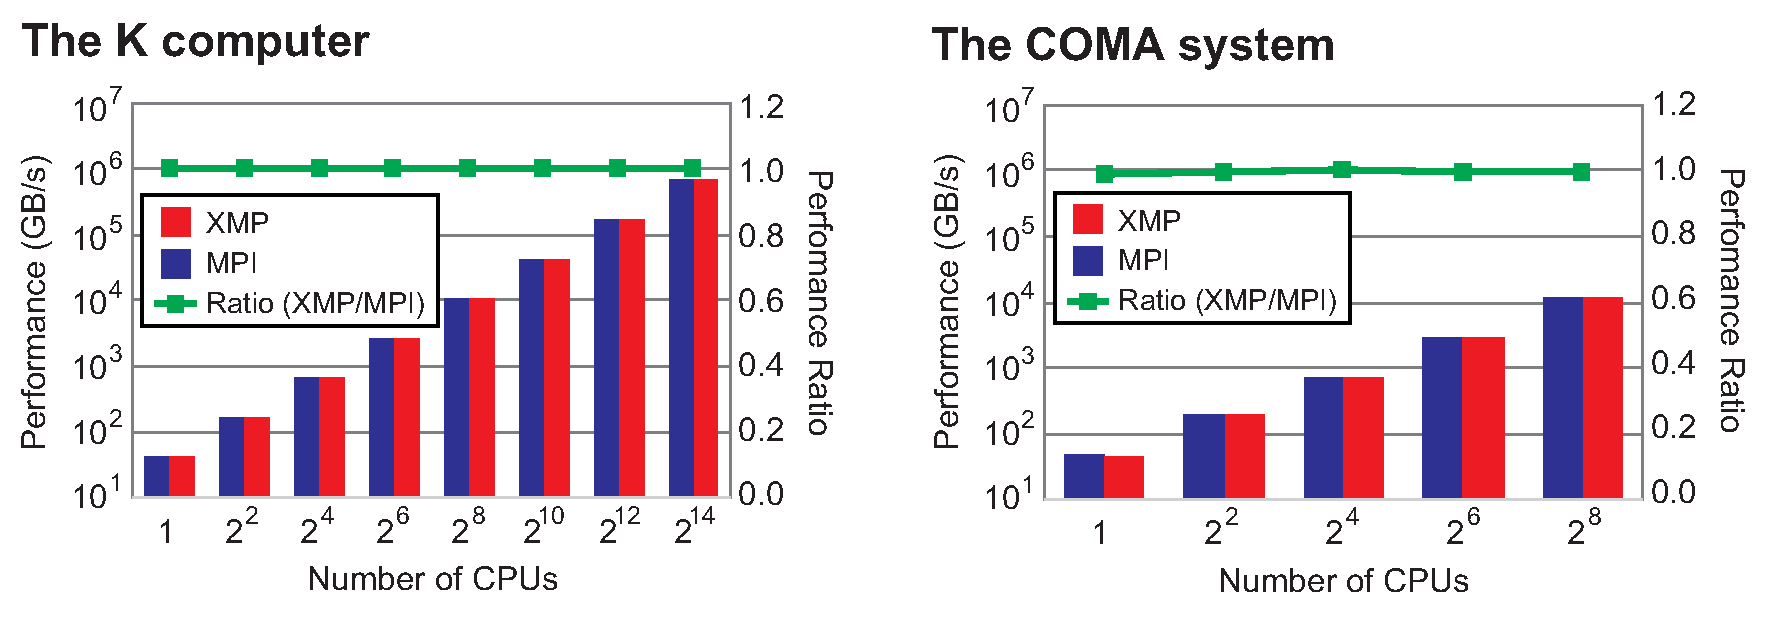
\includegraphics[scale=0.4,clip]{img/result-stream.eps}
\caption{Performance results for STREAM\cite{hpca}}\label{fig:result-stream}
\end{figure}

Fig.~\ref{fig:result-stream} shows the performance results and a comparative performance evaluation of both implementations.
The comparative performance evaluation is called the ``performance ratio''.
When the performance ratio is greater than 1,
the performance result of the XMP implementation is better than that of the MPI implementation.
XMP's best performance results are 706.38 TB/s for 16,384 compute nodes on the K computer,
and 11.55 TB/s for 128 compute nodes on the COMA system.
The values of the performance ratio are between 0.99 and 1.00 on both systems.
%%%%%%%%%%%%%%%%%%%%%%%%%%%%%%%%%%%%%%%%%%%%%%%%%%%%%%%%%%%%%%%%%%%%%%%%%%%%
\subsection{High Performance Linpack}
\subsubsection{Design}
HPL evaluates the floating point rate of execution for solving a linear system of equations. 
The performance result has been used in the TOP500 list (\url{\textcolor{blue}{https://www.top500.org}}).
To achieve a good load balance on HPL,
we distribute the main array in a {\it block-cyclic} manner.
Moreover, in order to achieve high performance with portability,
our implementation calls BLAS\cite{blas} to perform the matrix operations.
These techniques are inherited from the MPI implementation.

%%%%%%%%%%%%%%%%%%%%%%%%%%%%%%%%%%%%%%%%%%%%%%%%%%%%%%%%%%%%%%%%%%%%%%%%%%%%
\subsubsection{Implementation}
\begin{figure}[h]
\begin{lstlisting}
#pragma xmp template t[N][N]
#pragma xmp nodes p[Q][P]
#pragma xmp distribute t[cyclic(NB)][cyclic(NB)] onto p
double A[N][N];
#pragma xmp align A[i][j] with t[i][j]
\end{lstlisting}
%
\sidecaption
    
\includegraphics[scale=1.1,clip]{img/hpl-bc.eps}
    \caption{Block-cyclic distribution in HPL\cite{hpca}}\label{fig:hpl-bc}
\end{figure}

Fig.~\ref{fig:hpl-bc} shows that each dimension of the coefficient matrix {\it A[][]} is distributed in the {\it block-cyclic} manner.
The {\bf template} and the {\bf nodes} directives declare a two-dimensional template {\it t} and node array {\it p}.
The {\bf distribute} directive distributes {\it t} onto {\it Q} $\times$ {\it P} nodes with the same block size {\it NB}.
The {\bf align} directive aligns {\it A[][]} with {\it t}.

\begin{figure}[h]
    \begin{lstlisting}
double L[NB][N];
#pragma xmp align L[*][i] with t[*][i]
...
int len = N - j - NB;
#pragma xmp gmove async (tag)
L[0:NB][j+NB:len] = A[j:NB][j+NB:len];
    \end{lstlisting}
\sidecaption
    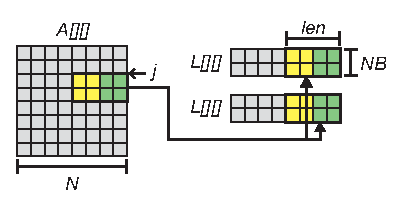
\includegraphics[scale=1.1,clip]{img/hpl-panel.eps}
    \caption{Panel broadcast in HPL\cite{hpca}}\label{fig:hpl-panel}
\end{figure}

HPL has an operation in which a part of the coefficient matrix is broadcast to the other process columns asynchronously.
This operation, called ``panel broadcast,'' is one of the most important operations for overlapping panel factorizations and data transfer.
Fig.~\ref{fig:hpl-panel} shows the implementation that uses the {\bf gmove} directive with the {\bf async} clause.
The second dimension of array {\it L[][]} is also distributed in a {\it block-cyclic} manner and {\it L[][]} is replicated.
%Thus, the {\bf gmove} directive performs such that elements {\it A[j:NB][j+NB:len][j:NB]}
%are \textcolor{blue}{broadcast} to {\it L[0:NB][j+NB:len]} asynchronously.
Thus, the {\bf gmove} directive broadcasts elements {\it A[j:NB][j+NB:len]} to {\it L[0:NB][j+NB:len]} asynchronously.

\begin{figure}[h]
\begin{lstlisting}
int L_ld, A_ld;
xmp_array_lda(xmp_desc_of(L), &L_ld);
xmp_array_lda(xmp_desc_of(A), &A_ld);
...
cblas_dgemm(..., &L[0][j], L_ld, ..., &A[i][j], A_ld, ...);
\end{lstlisting}
\caption{Calling the function {\bf cblas\_dgemm()} in HPL\cite{hpca}}\label{fig:hpl-dgemm}
\end{figure}

Fig.~\ref{fig:hpl-dgemm} shows that {\bf cblas\_dgemm()}, which is a BLAS function for a matrix multiplication,
applies the distributed arrays {\it L[][]} and {\it A[][]}.
Note that {\bf cblas\_dgemm()} is executed by multiple threads locally.
In lines 2--3,
{\bf xmp\_desc\_of()} gets descriptors of {\it L[][]} and {\it A[][]}, and
{\bf xmp\_array\_lda()} gets the leading dimensions {\it L\_ld} and {\it A\_ld}.
In line 5,
the {\it L\_ld} and {\it A\_ld} are used in {\bf cblas\_dgemm()}.
Note that {\it L\_ld} and {\it A\_ld} remain unchanged from the beginning of the program,
and so each {\bf xmp\_array\_lda()} is called only once.

\subsubsection{Evaluation}
\begin{figure}[h]
\sidecaption
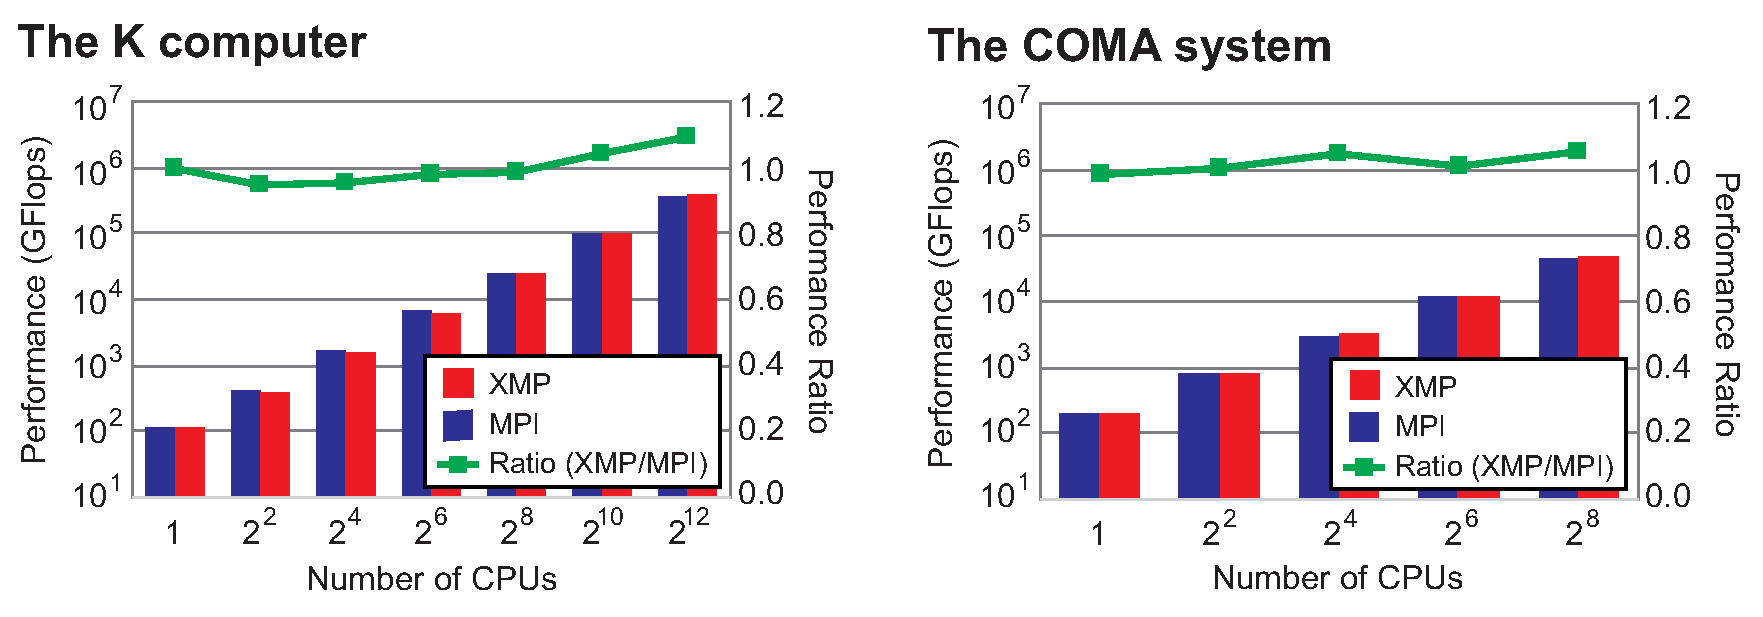
\includegraphics[scale=0.4,clip]{img/result-hpl.eps}
\caption{Performance results for HPL\cite{hpca}}\label{fig:result-hpl}
\end{figure}

Fig.~\ref{fig:result-hpl} shows the performance results and performance ratios.
XMP's best performance results are 402.01 TFlops (76.68\% of the peak performance) for 4,096 compute nodes on the K computer,
and 47.32 TFlops (70.02\% of the peak performance) for 128 compute nodes on the COMA system.
The values of the performance ratio are between 0.95 and 1.09 on the K computer,
and between 0.99 and 1.06 on the COMA system.

%%%%%%%%%%%%%%%%%%%%%%%%%%%%%%%%%%%%%%%%%%%%%%%%%%%%%%%%%%%%%%%%%%%%%%%%%%%%
\subsection{Global fast fourier transform}
\subsubsection{Design}
\begin{figure}[h]
\begin{lstlisting}
complex*16 a(4,12), b(12,4)
!$xmp template ty(12)
!$xmp template tx(4)
!$xmp nodes p(4)
!$xmp distribute ty(block) onto p
!$xmp distribute tx(block) onto p
!$xmp align a(*,i) with ty(i)
!$xmp align b(*,i) with tx(i)
call xmp_transpose(a, b, 1)
\end{lstlisting}
%
\begin{center}
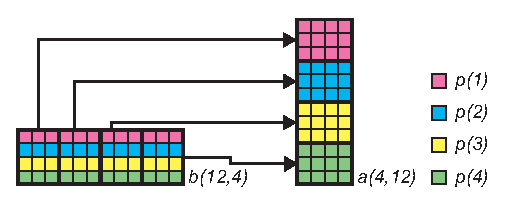
\includegraphics[scale=1.1,clip]{img/transpose.eps}
\caption{Action of subroutine {\bf xmp\_transpose()}\cite{hpca}}\label{fig:transpose}
\end{center}
\end{figure}

FFT evaluates the performance for a double-precision complex one-dimensional discrete fourier transform.
We implement a six-step FFT algorithm\cite{fft1, fft2} using FFTE library\cite{ffte}.
The six-step FFT algorithm is also used in the MPI implementation.
In the six-step FFT algorithm,
both the computing performance and the all-to-all communication performance for a matrix transpose are important.
The six-step FFT algorithm reduces the cache-miss ratio by expression of a two-dimensional array.
In order to develop the XMP implementation,
we use XMP in Fortran because FFTE library is written in Fortran and therefore it is easy to call it.
In addition, we use the XMP intrinsic subroutine {\bf xmp\_transpose()} to transpose a distributed array in the global-view memory model.
Fig.~\ref{fig:transpose} shows an example of {\bf xmp\_transpose()}.
The first argument is an output array, and the second argument is the input array.
The third argument is an option to save memory, and is ``0'' or ``1.''
If it is ``0,'' an input array must not be changed.
If it is ``1,'' an input array may be changed but less memory may be used.
Thus, we use ``1'' in the XMP implementation.
In Fig.~\ref{fig:transpose},
the second dimensions of arrays {\it a()} and {\it b()} are distributed in the {\it block} manner,
and array {\it b()} is transposed to array {\it a()}.
For example,
elements {\it b(1:3,2)} on {\it p(2)} are transferred to elements {\it a(2,1:3)} on {\it p(1)}.

%%%%%%%%%%%%%%%%%%%%%%%%%%%%%%%%%%%%%%%%%%%%%%%%%%%%%%%%%%%%%%%%%%%%%%%%%%%%
\subsubsection{Implementation}
\begin{figure}[h]
\begin{lstlisting}
complex*16 a(nx,ny), b(ny,nx), w(ny,nx)
!$xmp template ty(ny)
!$xmp template tx(nx)
!$xmp nodes p(*)
!$xmp distribute ty(block) onto p
!$xmp distribute tx(block) onto p
!$xmp align a(*,i) with ty(i)
!$xmp align b(*,i) with tx(i)
!$xmp align w(*,i) with tx(i)

integer, save :: ithread
!$omp threadprivate (ithread)
!$omp parallel
  ithread = omp_get_thread_num()
!$omp end parallel
!$xmp loop on tx(i)
!$omp parallel do
do i=1,nx
  call zfft1d(b(1,i),ny,-1,cy(1,ithread))
end do

!$xmp loop on tx(i)
!$omp parallel do
do i=1,nx
  do j=1,ny
    b(j,i)=b(j,i)*w(j,i)
  end do
end do

call xmp_transpose(a,b,1)
\end{lstlisting}
\caption{Part of the FFT code\cite{hpca}}\label{fig:code-fft}
\end{figure}

Fig.~\ref{fig:code-fft} shows a part of the XMP implementation.
In lines 1--9, arrays {\it a()}, {\it b()}, and {\it w()} are distributed in a {\it block} manner.
The {\it a()} is aligned with template {\it ty}, and the {\it b()} and {\it w()} arrays are aligned with template {\it tx}.
In lines 16--20, each thread on all nodes calls the FFTE subroutine {\it zfft1d()}, which applies the distributed array {\it b()}.
Note that the subroutine {\it zfft1d()} executes with a single thread locally.
In lines 22--23,
the XMP {\bf loop} directive and the OpenMP {\bf parallel} directive parallelize the loop statement.
In line 30, {\bf xmp\_transpose()} is used to transpose the distributed two-dimensional array.
%%%%%%%%%%%%%%%%%%%%%%%%%%%%%%%%%%%%%%%%%%%%%%%%%%%%%%%%%%%%%%%%%%%%%%%%%%%%
\subsubsection{Evaluation}
\begin{figure}[h]
\sidecaption
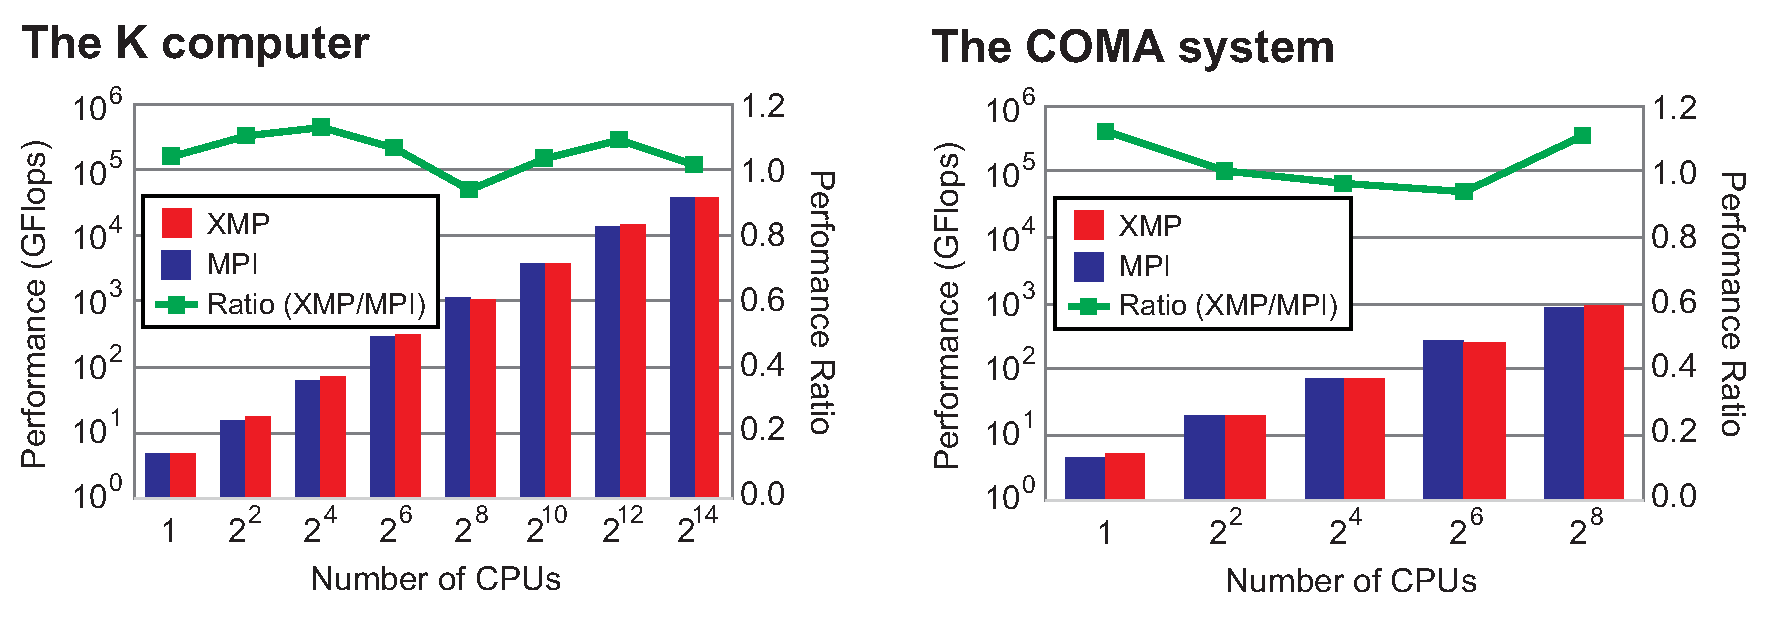
\includegraphics[scale=0.4,clip]{img/result-fft.eps}
\caption{Performance results for FFT\cite{hpca}}\label{fig:result-fft}
\end{figure}

Fig.~\ref{fig:result-fft} shows the performance results and performance ratios.
XMP's best performance results are 39.01 TFlops for 16,384 compute nodes on the K computer,
and 0.94 TFlops for 128 compute nodes on the COMA system.
The values of the performance ratio are between 0.94 and 1.13 on the K computer,
and between 0.94 and 1.12 on the COMA system.

%%%%%%%%%%%%%%%%%%%%%%%%%%%%%%%%%%%%%%%%%%%%%%%%%%%%%%%%%%%%%%%%%%%%%%%%%%%%
\subsection{RandomAccess}
\subsubsection{Design}
RandomAccess evaluates the performance of random updates of a single table of 64-bit integers which may be distributed among processes.
The random update for a distributed table requires an all-to-all communication.
We implement a recursive exchange algorithm\cite{randomaccess}, as with the MPI implementation.
The recursive exchange algorithm consists of multiple steps.
A process sends a data chunk to another process in each step.
Because RandomAccess requires a random communication pattern, as its name suggests,
the pattern is not supported by the global-view memory model.
Thus, we use the local-view memory model to implement RandomAccess.
Note that the MPI implementation uses functions {\bf MPI\_Isend()} and {\bf MPI\_Irecv()}.
%%%%%%%%%%%%%%%%%%%%%%%%%%%%%%%%%%%%%%%%%%%%%%%%%%%%%%%%%%%%%%%%%%%%%%%%%%%%

\subsubsection{Implementation}\label{sec:randomaccess}
A source node transfers a data chunk to a destination node,
and then the destination node updates own table using the received data.
The MPI implementation repeatedly executes the recursive exchange algorithm by 1,024 elements in the table.
The HPCC Award Competition class 2 specification defines the constant value 1,024.
The recursive exchange algorithm sends about half of the 1,024 elements in each step.
Therefore, the chunk size is about 4,096 Bytes ($= 1,024 / 2 \times 64 $ bits$ / 8 $).
%Since the same algorithm is used in both XMP and MPI implementations,
%the chunk size is also the same.
Note that the destination node cannot know how many elements are sent by the source node.
Thus, the MPI implementation gets the number of elements using the function {\bf MPI\_Get\_count()}.
We implement the algorithm using a coarray and the {\bf post}/{\bf wait} directives for the recursive exchange algorithm,
and the number of elements is added to the first element of the coarray.

\begin{figure}[h]
\begin{lstlisting}
#pragma xmp nodes p[*]
unsigned long long recv[ITER][LOGPROCS][CHUNK]:[*], send[2][CHUNKBIG]:[*];
...
for(j=0;j<logNumProcs;j++){
  ...
  send[i][0] = nsend;
  recv[iter_mod][j][0:nsend+1]:[ipartner] = send[i][0:nsend+1];
#pragma xmp post(p[ipartner], tag)
  ...
#pragma xmp wait(p[jpartner], tag)
  nrecv = recv[iter_mod][j-1][0];
  update_table(&recv[iter_mod][j-1][1], ..., nrecv, ...);
  ...
}
\end{lstlisting}
\caption{Part of the RandomAccess code\cite{hpca}}\label{fig:code-ra}
\end{figure}

Fig.~\ref{fig:code-ra} shows a part of the XMP implementation.
In line 2, the coarrays {\it recv[][][]} and {\it send[][]} are declared.
In line 6, the data chunk size is set at the first element of the coarray,
and it is put in line 7.
In line 8, the node sends notification of the completion of the coarray operation of line 7 to the node {\it p[ipartner]}.
In line 10, the node receives the notification from the node {\it p[jpartner]}, which ensures that the node {\it p[jpartner]} receives the data.
In line 11, the node gets the number of elements in the received data.
In line 12, the node updates own table by using the received data.
%%%%%%%%%%%%%%%%%%%%%%%%%%%%%%%%%%%%%%%%%%%%%%%%%%%%%%%%%%%%%%%%%%%%%%%%%%%%

\subsubsection{Evaluation}\label{sec:randomaccess-eva}
\begin{figure}[h]
\sidecaption
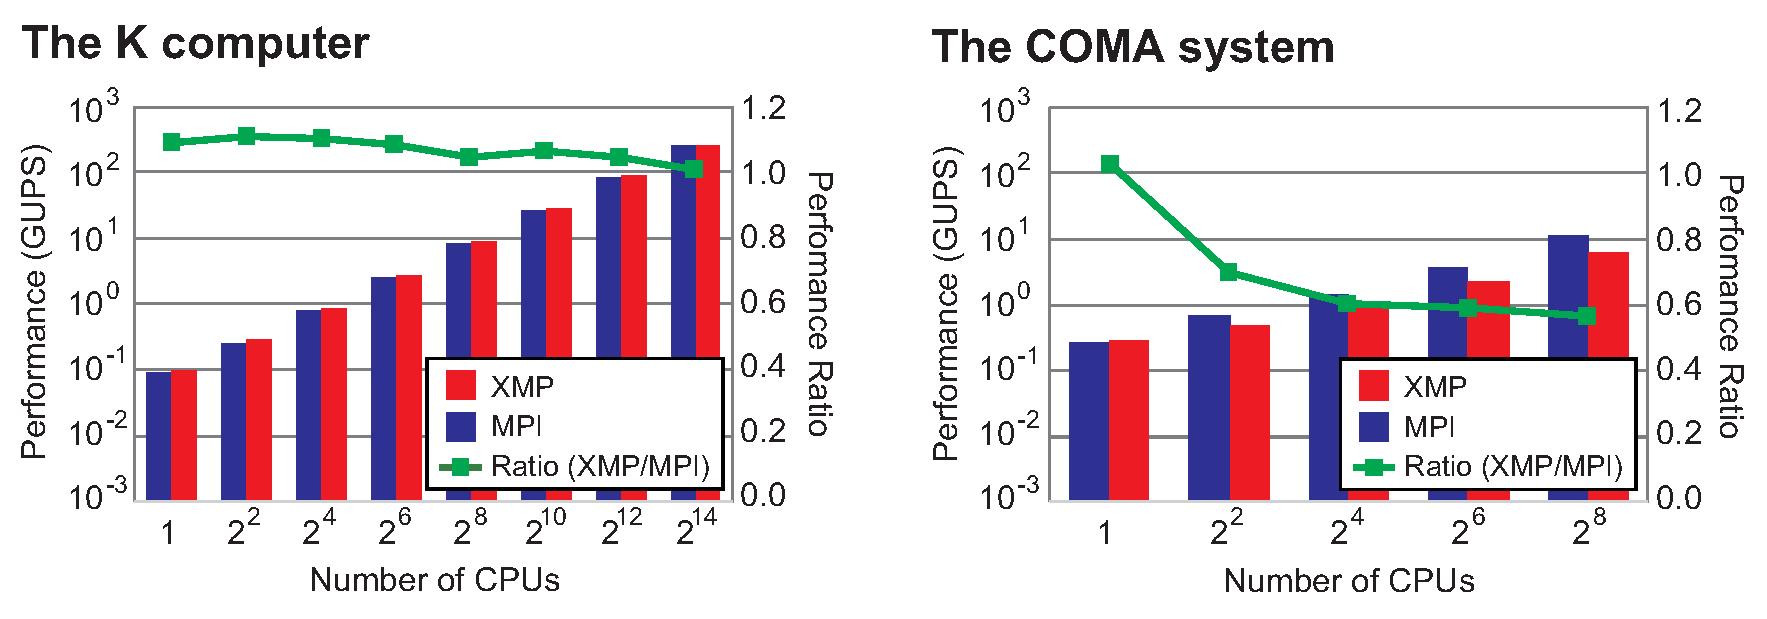
\includegraphics[scale=0.4,clip]{img/result-ra.eps}
\caption{Performance results for RandomAccess\cite{hpca}}\label{fig:result-ra}
\end{figure}

Fig.~\ref{fig:result-ra} shows the performance results and performance ratios.
The Giga-updates per second (GUPS) on the vertical axis is the measurement value, which is the number of update tables per second divided by $10^9$.
XMP's best performance results are 259.73 GUPS for 16,384 compute nodes on the K computer,
and 6.23 GUPS for 128 compute nodes on the COMA system.
The values of the performance ratio are between 1.01 and 1.11 on the K computer,
and between 0.57 and 1.03 on the COMA system.
On the K computer,
the performance results for the XMP implementation are always slightly better than those for the MPI implementation.
However, on the COMA system,
the performance results for the XMP implementation are worse than those for the MPI implementation using multiple CPUs.

%%%%%%%%%%%%%%%%%%%%%%%%%%%%%%%%%%%%%%%%%%%%%%%%%%%%%%%%%%%%%%%%%%%%%%%%%%%%
\subsection{Discussion}\label{sec:discussion}
We implement STREAM, HPL, and FFT using the global-view memory model, which
enables programmers to develop the parallel codes from the sequential codes using the XMP directives and functions easily.
Specifically, in order to implement the parallel STREAM code, a programmer only adds the XMP directives into the sequential STREAM code.
The XMP directives and existing directives, such as OpenMP directives and Fujitsu directives, can coexist.
Moreover, existing high-performance libraries, such as BLAS and FFTE, can be used with an XMP distributed array.
These features improve the portability and performance of XMP applications.

We also implement RandomAccess using the local-view memory model, where
the coarray syntax enables a programmer to transfer data intuitively.
In the evaluation,
the performance of the XMP implementation is better than that of the MPI implementation on the K computer,
but is worse than that of the MPI implementation on the COMA system.

To clarify the reason why XMP performance is dropped on the COMA system,
we develop a simple ping-pong benchmark using the local-view memory model.
The benchmark measures the latency for transferring data repeatedly between two nodes.
For comparison purposes, we also implement one using {\bf MPI\_Isend()} and {\bf MPI\_Irecv()} that are used in the MPI version RandomAccess.

\begin{figure}[h]
\begin{center}
\begin{lstlisting}
int me = xmpc_node_num();
int target = (me == 0)? 1 : 0;
...
if(me == 0){
  dst_buf[0:size]:[target] = src_buf[0:size];
#pragma xmp post(p[target], tag)
#pragma xmp wait(p[target], tag)
}
else if(me == 1){
#pragma xmp wait(p[target], tag)
  dst_buf[0:size]:[target] = src_buf[0:size];
#pragma xmp post(p[target], tag)
}
\end{lstlisting}
\end{center}

\begin{center}
\begin{lstlisting}
int me;
MPI_Comm_rank(..., &me);
int target = (me == 0)? 1 : 0;
...
if(me == 0){
  MPI_Isend(src_buf, ..., target, ...);
  MPI_Wait(...);
  MPI_Irecv(dst_buf, ..., target, ...);
  MPI_Wait(...);
}
else if(me == 1){
  MPI_Irecv(dst_buf, ..., target, ...);
  MPI_Wait(...);
  MPI_Isend(src_buf, ..., target, ...);
  MPI_Wait(...);
}
\end{lstlisting}
\end{center}
\caption{Part of the ping-pong benchmark code in XMP and MPI\cite{hpca}} \label{fig:pingpong-src}
\end{figure}


Fig.~\ref{fig:pingpong-src} shows parts of the codes.
In XMP of Fig.~\ref{fig:pingpong-src},
in line 5, {\it p[0]} puts a part of {\it src\_buf[]} into {\it dst\_buf[]} in {\it p[1]}.
In line 6, the {\bf post} directive ensures the completion of the coarray operation of line 5 and sends a notification to {\it p[1]}.
In line 10, {\it p[1]} waits until receiving the notification from {\it p[0]}.
In line 11, {\it p[1]} puts a part of {\it src\_buf[]} into {\it dst\_buf[]} in {\it p[0]}.
In line 12, the {\bf post} directive ensures the completion of the coarray operation of line 11 and sends a notification to {\it p[0]}.
In line 7, {\it p[0]} waits until receiving the notification from {\it p[1]}.
Fig.~\ref{fig:pingpong-src} also shows the ping-pong benchmark that uses MPI functions.

\begin{figure}[h]
\sidecaption
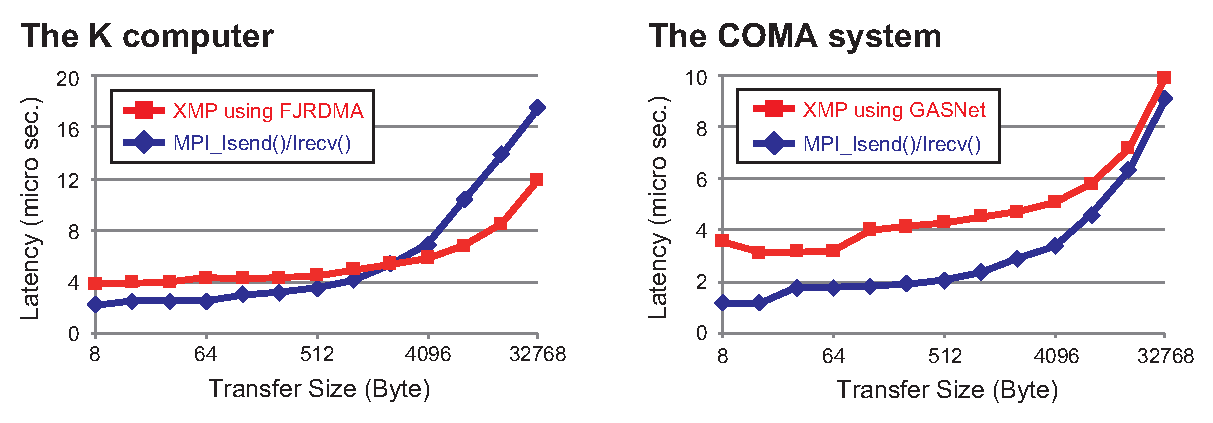
\includegraphics[scale=0.59,clip]{img/pingpong.eps}
\caption{Performance results for ping-pong benchmark\cite{hpca}}\label{fig:pingpong}
\end{figure}

Fig.~\ref{fig:pingpong} shows the latency for transferring data.
The results on the K computer show that
the latency for the XMP implementation is better than that for the MPI implementation for 2,048  Bytes or greater transfer size on the K computer.
In contrast,
the results on the COMA system show that
the latency of the XMP implementation is always worse than that of the MPI implementation on the COMA system.
The latency of XMP with FJRDMA at 4,096 Bytes, which is the average data chunk size, is 5.83 $\mu$s and
the latency of MPI is 6.89 $\mu$s on the K computer.
The latency of XMP with GASNet is 5.05 $\mu$s and
that of MPI is 3.37 $\mu$s on the COMA system.
Thus,
we consider the reason for the performance difference of RandomAccess is the communication performance.
The performance difference is also due to the differences in the synchronization mechanism of the one-sided XMP coarray and the two-sided MPI functions.
Note that a real application would not synchronize after every one-sided communication.
It is expected that a single synchronization should occur after multiple one-sided communications to achieve higher performance.

In addition,
the performance results for HPL and FFT are slightly different from those for the MPI implementations.
We consider that these differences are caused by small differences in the implementations.
In HPL, for the panel-broadcast operation,
the XMP implementation uses the {\bf gmove} directive with the {\bf async} clause, which calls {\bf MPI\_Ibcast()} internally.
In contrast,
the MPI implementation uses {\bf MPI\_Send()} and {\bf MPI\_Recv()} to perform the operation by the ``modified increasing ring''\cite{modified}.
In FFT, the XMP implementation uses XMP in Fortran, but the MPI implementation uses C language.
Both implementations call the same FFTE library.
In addition, the MPI implementation uses {\bf MPI\_Alltoall()} to transpose a matrix.
Since {\bf xmp\_transpose()} calls {\bf MPI\_Alltoall()} internally,
the performance levels for both {\bf xmp\_transpose()} and {\bf MPI\_Alltoall()} must be the same.
Therefore, the language differences and refactoring may have caused the performance difference.

%\subsection{Related work}\label{sec:relatedwork}
%\subsubsection{Implementations of the HPCC benchmark}
%The HPCC benchmark was implemented in some PGAS languages,
%such as XACC\cite{XACC1,XACC2},
%CAF 2.0\cite{caf-hpcc},
%Chapel\cite{2012Chapel-HPCC}, and
%X10\cite{2012X10-HPCC, Tardieu:2014:XAP:2555243.2555245}.

%XACC is an extension of XMP for an accelerated cluster system.
%XACC enables programmers to mix XMP and OpenACC directives to develop applications on the system.
%OpenACC provides directives for high performance, portability, and maintainability on a single compute node,
%and XACC can use the properties of OpenACC.
%Note that XACC is not a simple combination of XMP and OpenACC.
%XACC also supports new functions to develop accelerated applications easily.
%For example,
%XACC has a function to transfer data among accelerator memories directly.
%CAF 2.0 is an extension of the coarray features defined in Fortran 2008.
%For example,
%CAF 2.0 defines ``team'' as an image subset to set a range of communication,
%which is used for implementation of the panel-broadcast operation in HPL.
%Some of the features will be included in the next Fortran standard.
%and XMP will also include the fetures.

%PCJ is a library for Java language which provides functions for a task parallelism and one-sided communication through the global address space.
%The application using PCJ is run as typical Java application on Java Virtual Machine.

%Chapel and X10 are object-oriented languages funded by DARPA's High Productivity Computing Systems program.
%While Chapel has been developed by Cray Inc.,  X10 has been developed by IBM Research.
%An advantage of both Chapel and X10 is the support function for asynchronous task execution.
%The function is useful for developing a specific application, for example, an unbalanced tree search.
%While these are new languages, XMP is a language extension of C and Fortran.

%\subsubsection{Comparison with OpenMP and HPF}
%This section compares XMP to OpenMP and HPF, which are directive-based languages as XMP.
%OpenMP provides directives and library routines for parallel programming on shared memory systems,
%whereas XMP and HPF provide ones for distributed memory systems.
%OpenMP supports C, C++, and Fortran languages, whereas
%HPF is based only on Fortran.
%XMP is based on the C and Fortran languages, and so we also plan to support the C++ language as well as OpenMP.
%OpenMP uses the fork-join model as an execution model, whereas XMP uses the SPMD model.
%HPF does not use the SPMD model, which regards one virtual computer as multiple computers.
%OpenMP and HPF keep the semantics of the base code.
%XMP does not keep the semantics perfectly (e.g., the {\bf reflect} directive with {\bf periodic} clause)
%because of the improved performance and simplified parallelization.
%One of the biggest differences between HPF and XMP is that
%XMP enables programmers to perform explicit communication.
%The reason is that it is difficult to tune parallel applications by performing implicit communication with HPF\cite{Kennedy:2007:RFH:1238844.1238851}.
%In other words,
%while HPF's directives are hints for a compiler,
%XMP's directives define the actions of a compiler.

%%%%%%%%%%%%%%%%%%%%%%%%%%%%%%%%%%%%%%%%%%%%%%%%%%%%%%%%%%%%%%%%%%%%%%%%%%%%
\section{Conclusion}\label{sec:summary}
The chapter describes the  implementation and performance evaluation of Omni compiler.
We evaluate the performance of the HPCC benchmark in XMP on the K computer up to 16,384 compute nodes and a generic cluster system up to 128 compute nodes.
The performance results for the XMP implementations are almost the same as those for the MPI implementations in many cases.
Moreover, it demonstrates that the global-view and the local-view  memory models are useful to develop the HPCC benchmark.

%except for RandomAccess on a generic cluster system.

%%%%%%%%%%%%%%%%%%%%%%%% referenc.tex %%%%%%%%%%%%%%%%%%%%%%%%%%%%%%
% sample references
% %
% Use this file as a template for your own input.
%
%%%%%%%%%%%%%%%%%%%%%%%% Springer-Verlag %%%%%%%%%%%%%%%%%%%%%%%%%%
%
% BibTeX users please use
% \bibliographystyle{}
% \bibliography{}
%

\begin{thebibliography}{99.}%
% and use \bibitem to create references.
%
% Use the following syntax and markup for your references if 
% the subject of your book is from the field 
% "Mathematics, Physics, Statistics, Computer Science"
%
% Contribution 
\bibitem{caf} Robert W. Numrich and John Reid, ``Co-Array Fortran for
		parallel programming'', ACM SIGPLAN Fortran Forum, Vol.~17,
		No.~2 (1998).
\bibitem{upc} UPC Consortium, ``UPC Specifications, v1.2'', Lawrence
		Berkeley National Lab (LBNL-59208) (2005).
\bibitem{chapel} David Callahan, Bradford L.~Chamberlain and Hans
		P.~Zima,  ``The Cascade High Productivity Language'', Proc. 9th
		Int'l. Workshop on High-Level Parallel Programming Models and
		Supportive Environments (HIPS 2004), pp.~52--60 (2004).

\bibitem{ompt}
		{OpenMP Architecture Review Board}, ``OpenMP Application
		Programming Interface Version 5.0'' (2018).


\bibitem{MUST-project}
{The MUST Project},
\newblock https://www.itc.rwth-aachen.de/must.

\bibitem{Extrae-project}
{The Extrae Project},
\newblock https://tools.bsc.es/extrae.
%
% \bibitem{pro-env} Programming Environment Research Team.
% \url{https://pro-env.riken.jp}
% %
% \bibitem{hpcs} High Performance Computing System laboratory, University of Tsukuba, Japan.
% \url{https://www.hpcs.cs.tsukuba.ac.jp}
% %
% \bibitem{xcodeml} Mitsuhisa Sato et al.
%   ``Omni Compiler and XcodeML: An Infrastructure for Source-to-Source Transformation'',
%   Platform for Advanced Scientific Computing Conference (PASC16), Lausanne, Switzerland, Jun. (2016)
%  %
% \bibitem{ixpug} Masahiro Nakao et al.
%   ``Performance Evaluation for Omni XcalableMP Compiler on Many-core Cluster System based on Knights Landing'',
%   IXPUG Workshop Asia 2018, Tokyo, Japan, Jan. pp. 52--58 (2018)
% %
% \bibitem{github} \url{https://github.com/omni-compiler/omni-compiler}
% %
% %\bibitem{guide} \url{https://omni-compiler.org/manual/en/}
% %
% \bibitem{gasnet} \url{https://gasnet.lbl.gov}
% %
% \bibitem{scalasca} \url{https://www.scalasca.org}
% %
% \bibitem{hpcc} \url{https://icl.utk.edu/hpcc/}
% %
% \bibitem{hpca} Masahiro Nakao et al.
% ``Implementation and evaluation of the HPC Challenge benchmark in the XcalableMP PGAS language'',
%   International Journal of High Performance Computing Applications, 33(1), 110-123. Mar. (2017)
% %
% \bibitem{hpcc-a} \url{https://www.hpcchallenge.org}%
% %
% \bibitem{blas} BLAS: Basic Linear Algebra Subprograms \url{http://www.netlib.org/blas/} (2016)
% %
% \bibitem{fft1} David H. Bailey.
%   ``FFTs in external or hierarchical memory. Journal of Supercomputing'',
%   Vol.4, pp.23--35 (1990)
% %
% \bibitem{fft2} Van Loan C.
%   ``Computational Frameworks for the Fast Fourier Transform'',
%   Society for Industrial and Applied Mathematics (1992)
% %
% \bibitem{ffte} Daisuke Takahashi.
%   A Fast Fourier Transform Package. \url{http://www.ffte.jp} (2014)
% %
% \bibitem{randomaccess} Ponnusamy R. et al.
%   ``Communication overhead on the CM5: an experimental performance evaluation'',
%   Fourth Symposium on the Frontiers of Massively Parallel Computation, pp.108--115 (1992)
% %
% \bibitem{modified} HPL Algorithm Panel Broadcast. \url{http://www.netlib.org/benchmark/hpl/algorithm.html} (2016)
% %
% %\bibitem{XACC1} Masahiro Nakao et al.
% %  ``XcalableACC: Extension of XcalableMP PGAS Language Using OpenACC for Accelerator Clusters'',
% %  Proceedings of the First Workshop on Accelerator Programming Using Directives, pp.27--36 (2014)
% %
% %\bibitem{XACC2} Masahiro Nakao et al.
% %  ``Evaluation of XcalableACC with Tightly Coupled Accelerators/InfiniBand Hybrid Communication on Accelerated Cluster'',
% %  International Journal of High Performance Computing Applications, Jan. (2019)
% %
% %\bibitem{caf-hpcc} Guohua Jin et al.
% %  ``Implementation and Performance Evaluation of the HPC Challenge Benchmarks in Coarray Fortran 2.0'',
% %  Parallel Distributed Processing Symposium (IPDPS), 2011 IEEE International, pp.1089--1100 (2011)
% %
% %\bibitem{2012Chapel-HPCC} Brad Chamberlain et al.
% %  ``Chapel HPC Challenge Entry'',
% %  \url{http://www.hpcchallenge.org/presentations/sc2012/ChapelHPCC2012.pdf} (2011)
% %
% %\bibitem{2012X10-HPCC} Olivier Tardieu et al.
% %  ``X10 for Productivity and Performance at Scale'',
% %  \url{http://www.hpcchallenge.org/presentations/sc2012/x10-hpcc.pdf} (2012)
% %
% %\bibitem{Tardieu:2014:XAP:2555243.2555245} Olivier Tardieu et al.
% %  ``X10 and APGAS at Petascale'',
% %  Proceedings of the 19th ACM SIGPLAN Symposium on Principles and Practice of Parallel Programming pp.53--66 (2014)
% %
% %\bibitem{Kennedy:2007:RFH:1238844.1238851} Kennedy Ken et al.
% %  ``The rise and fall of High Performance Fortran: an historical object lesson'',
% %  Proceedings of the third ACM SIGPLAN conference on History of programming languages, pp.7-1--7-22 (2007)
% %
% %\bibitem{tsugane2016} Keisuke Tsugane et al.
% %  ``Proposal for Dynamic Task Parallelism in PGAS Language XcalableMP'',
% %  The 6th AICS International Symposium, p.57 (2016)
\end{thebibliography}

\end{document}
